\section{Experimental Details \& Further Discussion}\label{sec:appendix_experimental_details}

\subsection{Relational Games (\Cref{ssec:relgames})}\label{ssec:appendxi_relgames}

\subsubsection*{Experimental details}

\textbf{Dataset details.} The relational games benchmark datasets consists of $36 \times 36 \times 3$ RGB images depicting a $3 \times 3$ grid of objects which satisfy a particular visual relationship. The set of objects consists of simple geometric shapes. For example, in the \texttt{occurs} task, one object is present in the top row and three in the bottom row, and the task is to determine whether the object in the top row occurs (i.e., is among) the objects in the bottom row. The most difficult task in the benchmark is the \texttt{match pattern} task, where the grid contains a triplet of objects in the top row and another triplet of objects in the bottom row. Each triplet satisfies some relationship (e.g., ABC, ABA, ABB, or AAB), and the task is determine whether the relation in the first triplet is the same as the relation in the second triplet. The difficulty in solving this task is that it requires parsing a second-order relation (a relation between relations). We remark that composing relational attention modules naturally captures this kind of hierarchical relations: one relational attention operation produces objects with a relational representation and another would compute relations between those relations.

\textbf{Model architectures.} We use a Vision-Transformer-type architecture where the input image is split up into patches, flattened, and passed through the sequence model. We use average pooling at the end and pass through an MLP to produce the final prediction. We use a patch size of $12 \times 12$ which separates objects according to the grid structure. We note that in more general visual relational reasoning tasks where there isn't this type of grid structure, it would be appropriate to combine our approach with an object-discovery module such as Slot Attention~\citep{locatelloObjectCentricLearningSlot2020}.

We use the following hyperparameters: 2 layers, $\dmodel = 128$, $\dff = 128$, SwiGLU ``activation'', dropout rate = 0.1, pre-normalization. For the Orthrus models, we use positional symbols as the symbol assignment mechanism. The total number of heads is 2. For the Transformer model, there are only self-attention heads: $\nhsa = 2$. For Orthrus, we evaluated two configurations for the composition of head types, one with $\nhsa = 1, \nhra = 1$ and one with only relational attention heads $\nhsa = 0, \nhra = 2$. We also evaluated variants with and without the constraint that the relations in relational attention are symmetric (i.e., $\Wqrel = \Wkrel$).

\textbf{Training details.} For each task and model, we evaluated learning curves by varying the training set size and training the model until convergence, then evaluating on a hold-out test sets. For four out of five of the tasks, we evaluate learning curves within the range of $250$ to $2,500$ samples, in increments of $250$. For the more difficult \texttt{match pattern}, the range is from $5,000$ to $25,000$ in increments of $5,000$. The ranges were chosen based on the difficulty of the different tasks in order to identify the right ``resolution''. When evaluating learnign curves, each training set is sampled random from the full dataset. For each task, model, and training set size, we repeat the experiment 5 times with different random seeds to compute approximate confidence intervals (accounting for randomness in sampling the dataset and random initialization). We use an Adam optimizer with a learning rate of $0.001$, $\beta_1 = 0.9, \beta_2 = 0.99$, and a batch size of $512$. We train for 50 epochs.

\subsection*{Further Discussion, Exploration, \& Ablations}

We performed an ablation over the \textit{symmetry} inductive bias in the relations computed in relational attention. Our implementation exposes an argument which controls whether the relation $r(x, y) = (\iiprod{\Wqrell{\ell}}{\Wkrell{\ell}})_{\ell \in [d_r]} \in \reals^{d_r}$ modeled in relational attention is constrained to be symmetric by setting $\Wqrell{\ell} = \Wkrell{\ell}$. Indeed, we find symmetry to be a useful inductive bias in this task.~\Cref{fig:relgames_symmetry_ablation} depicts learning curves for the two configurations of Orthrus comparing symmetric DisRA against asymmetric DisRA. We find that symmetry results in faster learning curves for both configurations.

\begin{figure}
    \centering
    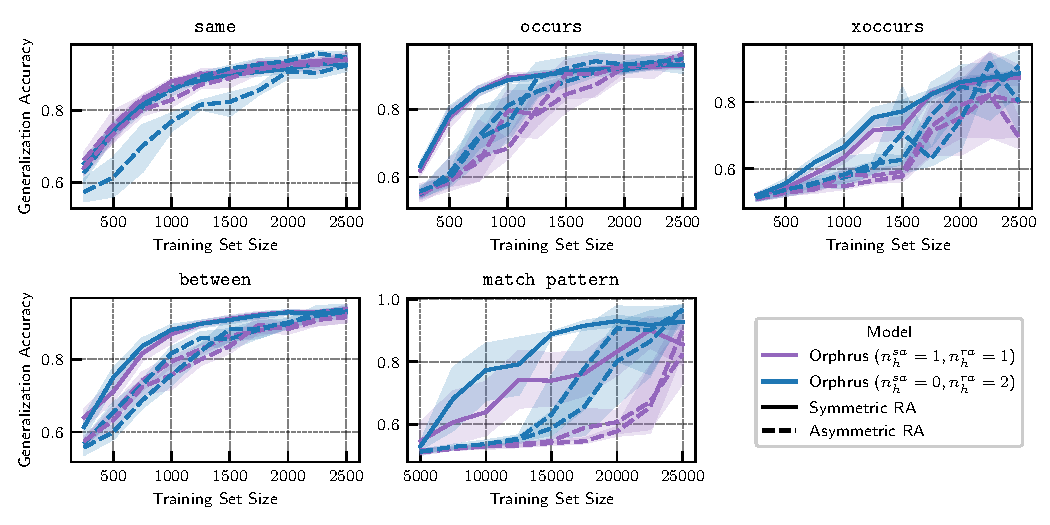
\includegraphics[width=\textwidth]{figs/experiments/relgames/relgames_learning_curves_symmetry_ablation.pdf}
    \caption{Ablation on effect of symmetry in relational attention.}\label{fig:relgames_symmetry_ablation}
\end{figure}

\aanote{TODO -- relgames symmetry ablation fig has two dashed lines. might be standard RCA. filter out.}

\subsection{Mathematical Problem-Solving (\Cref{ssec:math})}\label{ssec:appendix_math}

\begin{figure}
    \centering
    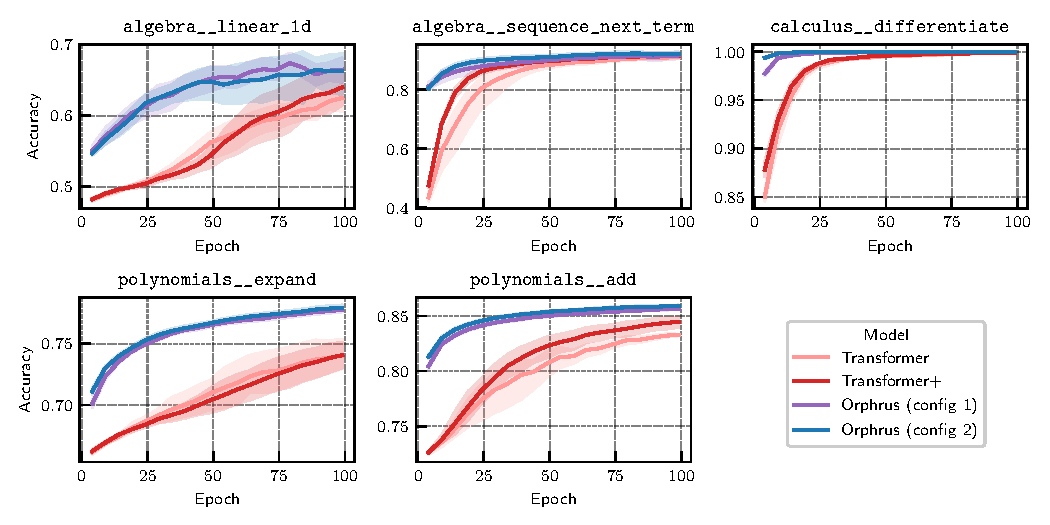
\includegraphics[width=\textwidth]{figs/experiments/math/math_training_curves_extrapolation.pdf}
    \caption{extrapolation accuracy curve}
\end{figure}

\begin{figure}
    \centering
    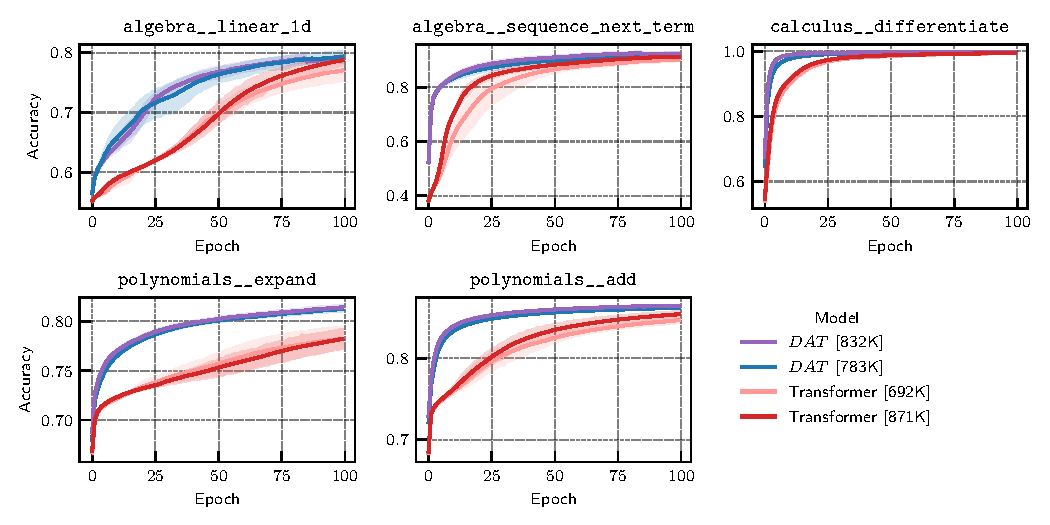
\includegraphics[width=\textwidth]{figs/experiments/math/math_training_curves_trainacc.pdf}
    \caption{Training accuracy curve}
\end{figure}
\aanote{need this? (math training acc curve)}


\subsection{Language Modeling (\Cref{ssec:tiny_stories})}\label{ssec:appendix_lm}

\begin{table}
    \caption{}\label{tab:}
    
\begin{tabular}{@{}|c|c|c|c|c|c|c|c|@{}}
\toprule
$\dmodel$             & $L$                & $\nhsa$            & $\nhra$            & Symbol Assignment Mechanism                & Symmetric RA & val/loss       & val/perplexity \\
\midrule
\multirow{23}{*}{64}  & \multirow{9}{*}{4} & \multirow{4}{*}{4} & \multirow{4}{*}{4} & \multirow{2}{*}{Position-Relative Symbols} & False        & 1.764          & 5.840          \\
                        &                    &                    &                    &                                            & True         & 1.785          & 5.963          \\ \cline{5-8} 
                        &                    &                    &                    & \multirow{2}{*}{Symbolic Attention}        & False        & \textbf{1.729} & \textbf{5.639} \\
                        &                    &                    &                    &                                            & True         & 1.744          & 5.722          \\ \cline{3-8} 
                        &                    & \multirow{4}{*}{6} & \multirow{4}{*}{2} & \multirow{2}{*}{Position-Relative Symbols} & False        & 1.768          & 5.859          \\
                        &                    &                    &                    &                                            & True         & 1.777          & 5.914          \\ \cline{5-8} 
                        &                    &                    &                    & \multirow{2}{*}{Symbolic Attention}        & False        & 1.740          & 5.697          \\
                        &                    &                    &                    &                                            & True         & 1.745          & 5.727          \\ \cline{3-8} 
                        &                    & 8                  & 0                  & NA                                         & NA           & 1.775          & 5.903          \\ \cline{2-8} 
                        & \multirow{6}{*}{5} & \multirow{2}{*}{4} & \multirow{2}{*}{4} & \multirow{2}{*}{Symbolic Attention}        & False        & \textbf{1.692} & \textbf{5.431} \\
                        &                    &                    &                    &                                            & True         & 1.698          & 5.467          \\ \cline{3-8} 
                        &                    & \multirow{3}{*}{6} & \multirow{3}{*}{2} & Position-Relative Symbols                  & True         & 1.730          & 5.640          \\ \cline{5-8} 
                        &                    &                    &                    & \multirow{2}{*}{Symbolic Attention}        & False        & \textbf{1.692} & \textbf{5.432} \\
                        &                    &                    &                    &                                            & True         & 1.704          & 5.495          \\ \cline{3-8} 
                        &                    & 8                  & 0                  & NA                                         & NA           & 1.730          & 5.640          \\ \cline{2-8} 
                        & \multirow{8}{*}{6} & \multirow{4}{*}{4} & \multirow{4}{*}{4} & \multirow{2}{*}{Position-Relative Symbols} & False        & 1.685          & 5.395          \\
                        &                    &                    &                    &                                            & True         & 1.704          & 5.498          \\ \cline{5-8} 
                        &                    &                    &                    & \multirow{2}{*}{Symbolic Attention}        & False        & \textbf{1.656} & \textbf{5.239} \\
                        &                    &                    &                    &                                            & True         & 1.668          & 5.303          \\ \cline{3-8} 
                        &                    & \multirow{3}{*}{6} & \multirow{3}{*}{2} & Position-Relative Symbols                  & True         & 1.691          & 5.424          \\ \cline{5-8} 
                        &                    &                    &                    & \multirow{2}{*}{Symbolic Attention}        & False        & 1.663          & 5.277          \\
                        &                    &                    &                    &                                            & True         & 1.669          & 5.308          \\ \cline{3-8} 
                        &                    & 8                  & 0                  & NA                                         & NA           & 1.692          & 5.431          \\ \hline
\multirow{10}{*}{128}   & \multirow{5}{*}{4} & \multirow{2}{*}{4} & \multirow{2}{*}{4} & \multirow{2}{*}{Symbolic Attention}        & False        & \textbf{1.411} & \textbf{4.102} \\
                        &                    &                    &                    &                                            & True         & 1.417          & 4.127          \\ \cline{3-8} 
                        &                    & \multirow{2}{*}{6} & \multirow{2}{*}{2} & \multirow{2}{*}{Symbolic Attention}        & False        & 1.412          & 4.105          \\
                        &                    &                    &                    &                                            & True         & 1.415          & 4.118          \\ \cline{3-8} 
                        &                    & 8                  & 0                  & NA                                         & NA           & 1.431          & 4.183          \\ \cline{2-8} 
                        & \multirow{5}{*}{6} & \multirow{2}{*}{4} & \multirow{2}{*}{4} & \multirow{2}{*}{Symbolic Attention}        & False        & \textbf{1.337} & \textbf{3.811} \\
                        &                    &                    &                    &                                            & True         & 1.346          & 3.843          \\ \cline{3-8} 
                        &                    & \multirow{2}{*}{6} & \multirow{2}{*}{2} & \multirow{2}{*}{Symbolic Attention}        & False        & 1.340          & \textbf{3.818} \\
                        &                    &                    &                    &                                            & True         & 1.346          & 3.843          \\ \cline{3-8} 
                        &                    & 8                  & 0                  & NA                                         & NA           & 1.353          & 3.870          \\ \bottomrule
\end{tabular}%
\end{table}
\aanote{todo--fix table formatting and add missing / remove incomplete runs}

\begin{figure}
    \centering
    \begin{subfigure}{0.45\textwidth}
        \centering
        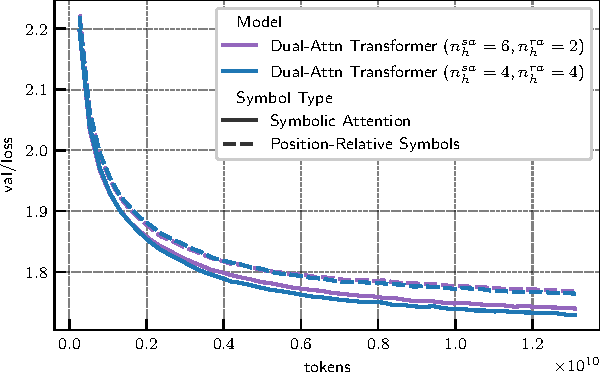
\includegraphics[width=\textwidth]{figs/experiments/tiny_stories/d64L4_ablation_symboltype_asymra.pdf}
        \caption{$d=64, L=4$, asymmetric RA}
    \end{subfigure}
    \begin{subfigure}{0.45\textwidth}
        \centering
        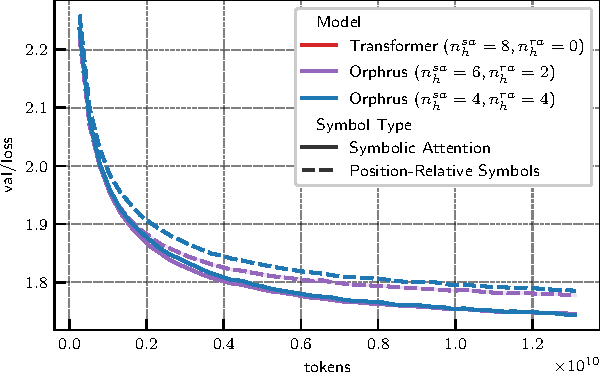
\includegraphics[width=\textwidth]{figs/experiments/tiny_stories/d64L4_ablation_symboltype_symra.pdf}
        \caption{$d=64, L=4$, symmetric RA}
    \end{subfigure}
    \caption{Ablation of symbol type}
\end{figure}

\begin{figure}
    \centering
    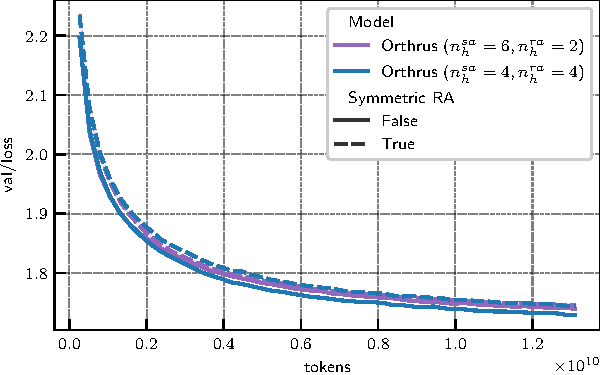
\includegraphics[width=0.5\textwidth]{figs/experiments/tiny_stories/d64L4_ablation_symmetry_symmattn.pdf}
    \caption{Ablation of symbol type}
\end{figure}

% add figure with d=128, L=4, 6